\documentclass[a4paper]{article}

\usepackage{INTERSPEECH_v2}
\usepackage{fancyvrb}
\usepackage{relsize}
\usepackage{url}
\usepackage{balance}

\DeclareMathOperator*{\argmax}{arg\,max}

\title{\texttt{\Large{pyannote.metrics}}: a toolkit for reproducible evaluation,\\ diagnostic, and error analysis of speaker diarization systems}
\name{Herv\'{e} Bredin}
\address{
  LIMSI, CNRS, Universit\'{e} Paris-Saclay, France}
\email{bredin+pyannote@limsi.fr}

\begin{document}

\maketitle
%
\begin{abstract}
\texttt{pyannote.metrics} is an open-source Python library aimed at researchers working in the wide area of speaker diarization.
It provides a command line interface (CLI) to improve reproducibility and comparison of speaker diarization research results. Through its application programming interface (API), a large set of evaluation metrics is available for diagnostic purposes of all modules of typical speaker diarization pipelines (speech activity detection, speaker change detection, clustering, and identification). Finally, thanks to visualization capabilities, we show that it can also be used for detailed error analysis purposes. \texttt{pyannote.metrics} can be downloaded from \url{pyannote.github.io}.
\end{abstract}
\noindent\textbf{Index Terms}: evaluation, speaker diarization, reproducible research, open-source software

\section{Introduction}

Speaker diarization is the task of partitioning an audio stream into homogeneous temporal segments according to the identity of the speaker.
Automatic speech transcription also benefits from speaker diarization to address the question ``who speaks what?''.
Resulting augmented (or ``rich'') transcription can be very useful for multimedia documents structuring and indexing.

Thanks to open initiatives such as the series of NIST ``Rich Transcription'' evaluations~\cite{Fiscus2006}, or ESTER~\cite{Galliano2005} and  ETAPE~\cite{Gravier2012} benchmarks, the state-of-the-art for speaker diarization has achieved significant improvement since 2000.
Despite addressing the same task, these initiatives used different evaluation metrics, different implementations of these metrics~\cite{NIST-RT03, Galibert2013}, all provided as standalone (C or Lua) command line tools.

In this paper, we introduce \texttt{pyannote.metrics}, an open-source Python library for reproducible evaluation, diagnostic, and error analysis of speaker diarization systems.
Python is currently being adopted by a growing number of researchers in speaker identification~\cite{sidekit, Bob2012}, machine learning~\cite{scikit-learn}, or deep learning~\cite{tensorflow2015-whitepaper}.
Being able to directly evaluate speaker diarization using the computer language in which systems are developed is therefore very convenient.

\begin{figure*}[htb]
  \centering
  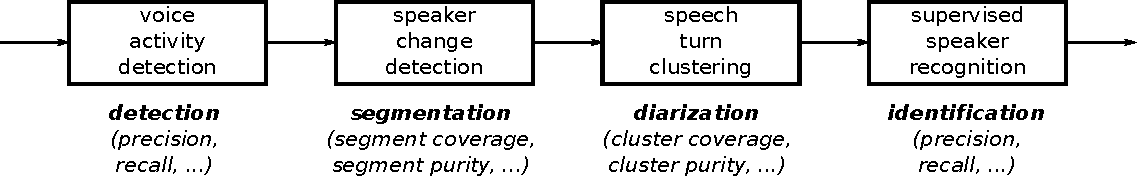
\includegraphics[width=0.8\linewidth]{figures/pipeline.pdf}
  \caption{A typical pipeline for speaker diarization, aligned with the list of available evaluation metrics }
  \label{fig:pipeline}
\end{figure*}

As introduced in Section~\ref{sec:reproducible_evaluation}, \texttt{pyannote.metrics} can be used as a command line tool to compute the \emph{de facto} standard \emph{diarization error rate} NIST implementation.
Inspired by Bob~\cite{Bob2012} database package paradigm, \texttt{pyannote.metrics} rely on standardized database interfaces to ensure reproducibility and fair comparison of speaker diarization systems.
It also provides a large collections of additional evaluation metrics (summarized in Figure~\ref{fig:pipeline}) that can be used for diagnostic purposes, either using the command line tool, or directly as a Python module.
Those additional metrics are described, discussed, and compared in Section~\ref{sec:diagnostic}.
Finally, another strength of \texttt{pyannote.metrics} lies in its advanced visualization and error analysis features.
This is introduced in Section~\ref{sec:visualization}.

\section{Reproducible evaluation}
\label{sec:reproducible_evaluation}

There are two main issues that may arise with results reported in the literature.
Firstly, even though the same public datasets are used, the actual evaluation protocol may differ slightly from one paper to another.
Secondly, the implementation of the reported evaluation metrics may also differ.
The first objective of the \texttt{pyannote.metrics} library is to address these two problems, and provide a convenient way for researchers to evaluate their approaches in a reproducible and comparable manner.
Figure~\ref{vrb:cli} shows an example use of the command line interface that is provided to solve this problem.

\begin{figure*}[htb]
\begin{Verbatim}[showspaces=false,fontsize=\relsize{-1}]
$ pyannote.metrics.py diarization --subset=development Etape.SpeakerDiarization.TV hypothesis.mdtm
\end{Verbatim}
\begin{Verbatim}[showspaces=false,fontsize=\relsize{-3}]
Diarization (collar = 0 ms)               error    purity    coverage     total    correct      %    fa.      %    miss.     %    conf.      %
--------------------------------------  -------  --------  ----------  --------  ---------  -----  ------  -----  -------  ----  -------  -----
BFMTV_BFMStory_2011-03-17_175900          14.64     94.74       90.00   2582.08    2300.22  89.08   96.16   3.72    80.14  3.10   201.72   7.81
LCP_CaVousRegarde_2011-02-17_204700       17.80     89.13       86.90   3280.72    2848.42  86.82  151.78   4.63   208.29  6.35   224.01   6.83
LCP_EntreLesLignes_2011-03-18_192900      23.46     79.52       79.03   1704.97    1337.80  78.46   32.89   1.93   157.14  9.22   210.03  12.32
LCP_EntreLesLignes_2011-03-25_192900      26.75     76.97       75.86   1704.13    1292.83  75.86   44.61   2.62   158.38  9.29   252.92  14.84
LCP_PileEtFace_2011-03-17_192900          10.73     93.33       92.30   1611.49    1487.32  92.30   48.73   3.02    55.49  3.44    68.67   4.26
LCP_TopQuestions_2011-03-23_213900        18.28     98.25       94.20    727.26     668.65  91.94   74.36  10.22    16.41  2.26    42.20   5.80
LCP_TopQuestions_2011-04-05_213900        27.97     97.95       79.81    818.03     638.68  78.08   49.45   6.04    17.46  2.13   161.89  19.79
TV8_LaPlaceDuVillage_2011-03-14_172834    21.43     92.89       89.64    996.12     892.04  89.55  109.36  10.98    11.80  1.18    92.28   9.26
TV8_LaPlaceDuVillage_2011-03-21_201334    66.23     77.24       70.64   1296.86     691.76  53.34  253.80  19.57    29.16  2.25   575.95  44.41
TOTAL                                     23.27     88.18       84.55  14721.65   12157.71  82.58  861.14   5.85   734.28  4.99  1829.67  12.43
\end{Verbatim}
\caption{\small{\texttt{pyannote-metrics.py}} example output}
\label{vrb:cli}
\end{figure*}

\subsection{Multiple tasks}

The first positional argument (\emph{e.g.} \texttt{diarization} in Figure~\ref{vrb:cli}) is a flag indicating which task should be evaluated.
Apart for the \texttt{diarization} flag that is used for evaluating speaker diarization results, other available flags are \texttt{detection} (speech activity detection), \texttt{segmentation} (speaker change detection), and \texttt{identification} (supervised speaker identification).
These four flags correspond to the typical four modules used in  most speaker diarization systems, as depicted in Figure~\ref{fig:pipeline}.
Depending on the task, a different set of evaluation metrics is computed, which are listed in Section~\ref{sec:diagnostic}.

\subsection{Multiple datasets and protocols}

The second positional argument, along with the optional \texttt{--subset} argument, provides an easy way to ensure the same protocol (\emph{i.e.} manual groundtruth and training/development/test split) is used for evaluation.
Internally, it relies on a collection of Python packages that all derive from the \texttt{pyannote.database} main package, that provides a convenient API to define training/development/test splits, along with groundtruth annotations.
As of March 2017, \texttt{pyannote.database} packages exist for the ETAPE corpus~\cite{Gravier2012}, the REPERE corpus~\cite{giraudel_repere_2012, galibert_first_2013}, and the AMI corpus~\cite{Carletta2007}.
As more people contribute new \texttt{pyannote.database} packages, they will be added to the \texttt{pyannote} ecosystem.
In Figure~\ref{vrb:cli}, the development set of the \emph{TV} evaluation protocol of the ETAPE dataset is used.
Results are both reported for each file in the selected subset, and aggregated into one final metric value (\emph{cf.} line starting with \texttt{TOTAL}).

\subsection{Multiple supported formats}

The final positional argument is the path to the file that contains the output of the evaluated speaker diarization system.
While the \texttt{MDTM}~\cite{NIST-RT03} file format is used in this example, several other file formats are available (and can be contributed) thanks to the internal use of the \texttt{pyannote.parser} package.

\section{Diagnostic}
\label{sec:diagnostic}

A typical speaker diarization pipeline is depicted in Figure~\ref{fig:pipeline}.
The first step is usually dedicated to speech activity detection, where the objective is to get rid of all non-speech regions.
Then, speaker change detection aims at segmenting speech regions into homogeneous segments.
The subsequent clustering step tries to group those speech segments according to the identity of the speaker.
Finally, an optional supervised classification step may be applied to actually identity every speaker cluster in a supervised way.

Looking at the final performance of the system is usually not enough for diagnostic purposes.
In particular, it is often necessary to evaluate the performance of each module separately to identify their strenght and weakness, or to estimate the influence of their errors on the complete pipeline.
This section provides the list of metrics that were implemented in \texttt{pyannote.metrics} with that very goal in mind.

\subsection{Detection}

Speech activity detection modules can be evaluated using, detection error rate, precision, and recall.

\begin{equation}
  \text{detection error rate} = \frac{\text{false alarm} + \text{missed detection}}{\text{total}}
\end{equation}
where $\text{false alarm}$ is the duration of non-speech incorrectly classified as speech, $\text{missed detection}$ is the duration of
speech incorrectly classified as non-speech, and $\text{total}$ is the total duration of speech in the reference.
Note that these metrics do not take overlapping speech into account.
In other words, overlapping speech regions are counted only once.

\subsection{Segmentation}

\begin{figure}[htb]
  \centering
  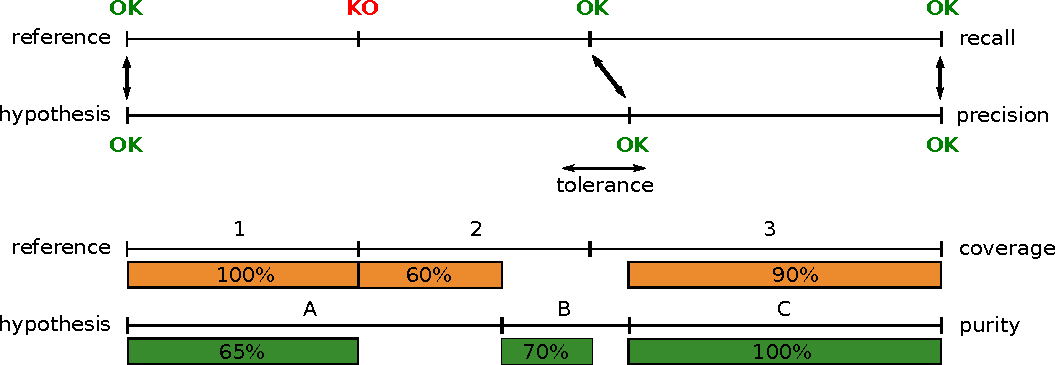
\includegraphics[width=1.0\linewidth]{figures/segmentation.pdf}
  \caption{Segmentation metrics available in \texttt{pyannote.metrics}}
  \label{fig:segmentation}
\end{figure}

As depicted in Figure~\ref{fig:segmentation}, (speaker) change detection modules can be evaluated using two pairs of dual metrics: precision and recall, or purity and coverage. Precision and recall are standard metrics based on the number of correctly detected speaker boundaries. In Figure~\ref{fig:segmentation}, recall is $75\%$ because 3 out of 4 reference boundaries were correctly detected, and precision is $100\%$ because all hypothesized boundaries are correct. The main weakness of that pair of metrics (and their combination into a f-score) is that it is very sensitive to the \emph{tolerance} parameter, \emph{i.e.} the maximum distance between two boundaries for them to be matched. From one segmentation paper to another, authors may used very different values, thus making the approaches difficult to compare.

Instead, we think that segment-wise purity and coverage should be used instead.
They have several advantages over precision and recall, including the fact that they do not depend on any \emph{tolerance} parameter, and that they directly relate to the cluster-wise purity and coverage used for evaluating speaker diarization.
Segment-wise coverage is computed for each segment in the reference as the ratio of the duration of the intersection with the most co-occurring hypothesis segment and the duration of the reference segment. For instance, coverage for reference segment 1 is $100\%$ because it is entirely covered by hypothesis segment A. Purity is the dual metric that indicates how \emph{pure} hypothesis segments are. For instance, segment A is only $65\%$ pure because it is covered at $65\%$ by segment 1 and $35\%$ by segment 2.
The final values are duration-weighted average over each segment.

\subsection{Diarization}

Diarization error rate (DER) is the \emph{de facto} standard metric for evaluating and comparing speaker diarization systems.
It is defined as follows:

\begin{equation*}
  \text{DER} = \frac{\text{false alarm} + \text{missed detection} + \text{confusion}}{\text{total}}
\end{equation*}
where $\text{false alarm}$ is the duration of non-speech incorrectly classified as speech, $\text{missed detection}$ is the duration of
speech incorrectly classified as non-speech, $\text{confusion}$ is the duration of speaker confusion, and $\text{total}$ is the total duration of speech in the reference.
Note that this metric does take overlapping speech into account, potentially leading to increased missed detection in case the speaker diarization system does not include an overlapping speech detection module.

\subsubsection{``Optimal'' \emph{vs.} ``greedy''}

Two implementations of the diarization error rate are available (optimal and greedy), depending on how the one-to-one mapping between reference and hypothesized speakers is computed.
The \emph{optimal} version uses the Hungarian algorithm~\cite{Kuhn1955} to compute the mapping that minimize the $\texttt{confusion}$ term, while the \emph{greedy} version operates in a greedy manner, mapping reference and hypothesized speakers iteratively, by decreasing value of their cooccurrence duration.
In practice, the \emph{greedy} version is much faster than the \emph{optimal} one, especially for files with a large number of speakers -- though it may slightly over-estimate the value of the diarization error rate.

\subsubsection{Purity and coverage}

While the diarization error rate provides a convenient way to compare different diarization approaches, it is usually not enough to understand the type of errors commited by the system.
Purity~\cite{cettolo2000segmentation} and coverage~\cite{gauvain1998partitioning} are two dual evaluation metrics that provide additional insight on the behavior of the system.
They are defined as follows:

\begin{eqnarray*}
   \text{purity} & = & \frac{\displaystyle \sum_{\text{cluster}} \max_{\text{speaker}} |\text{cluster} \cap \text{speaker}|  }{\displaystyle \sum_{\text{cluster}} |\text{cluster}|} \\
  \text{coverage} & = & \frac{\displaystyle \sum_{\text{speaker}} \max_{\text{cluster}} |\text{speaker} \cap \text{cluster}|  }{\displaystyle \sum_{\text{speaker}} |\text{speaker}|} \\
\end{eqnarray*}
where $|\text{speaker}|$ (respectively $|\text{cluster}|$ is the speech duration of this particular reference speaker (resp. hypothesized cluster), and  $|\text{speaker} \cap \text{cluster}|$ is the duration of their intersection.
Over-segmented results (\emph{e.g.} too many speaker clusters) tend to lead to high purity and low coverage, while under-segmented results (\emph{e.g.} when two speakers are merged into one large cluster) lead to low purity and higher coverage.

\subsubsection{Use case}

\begin{figure}[htb]
  \centering
  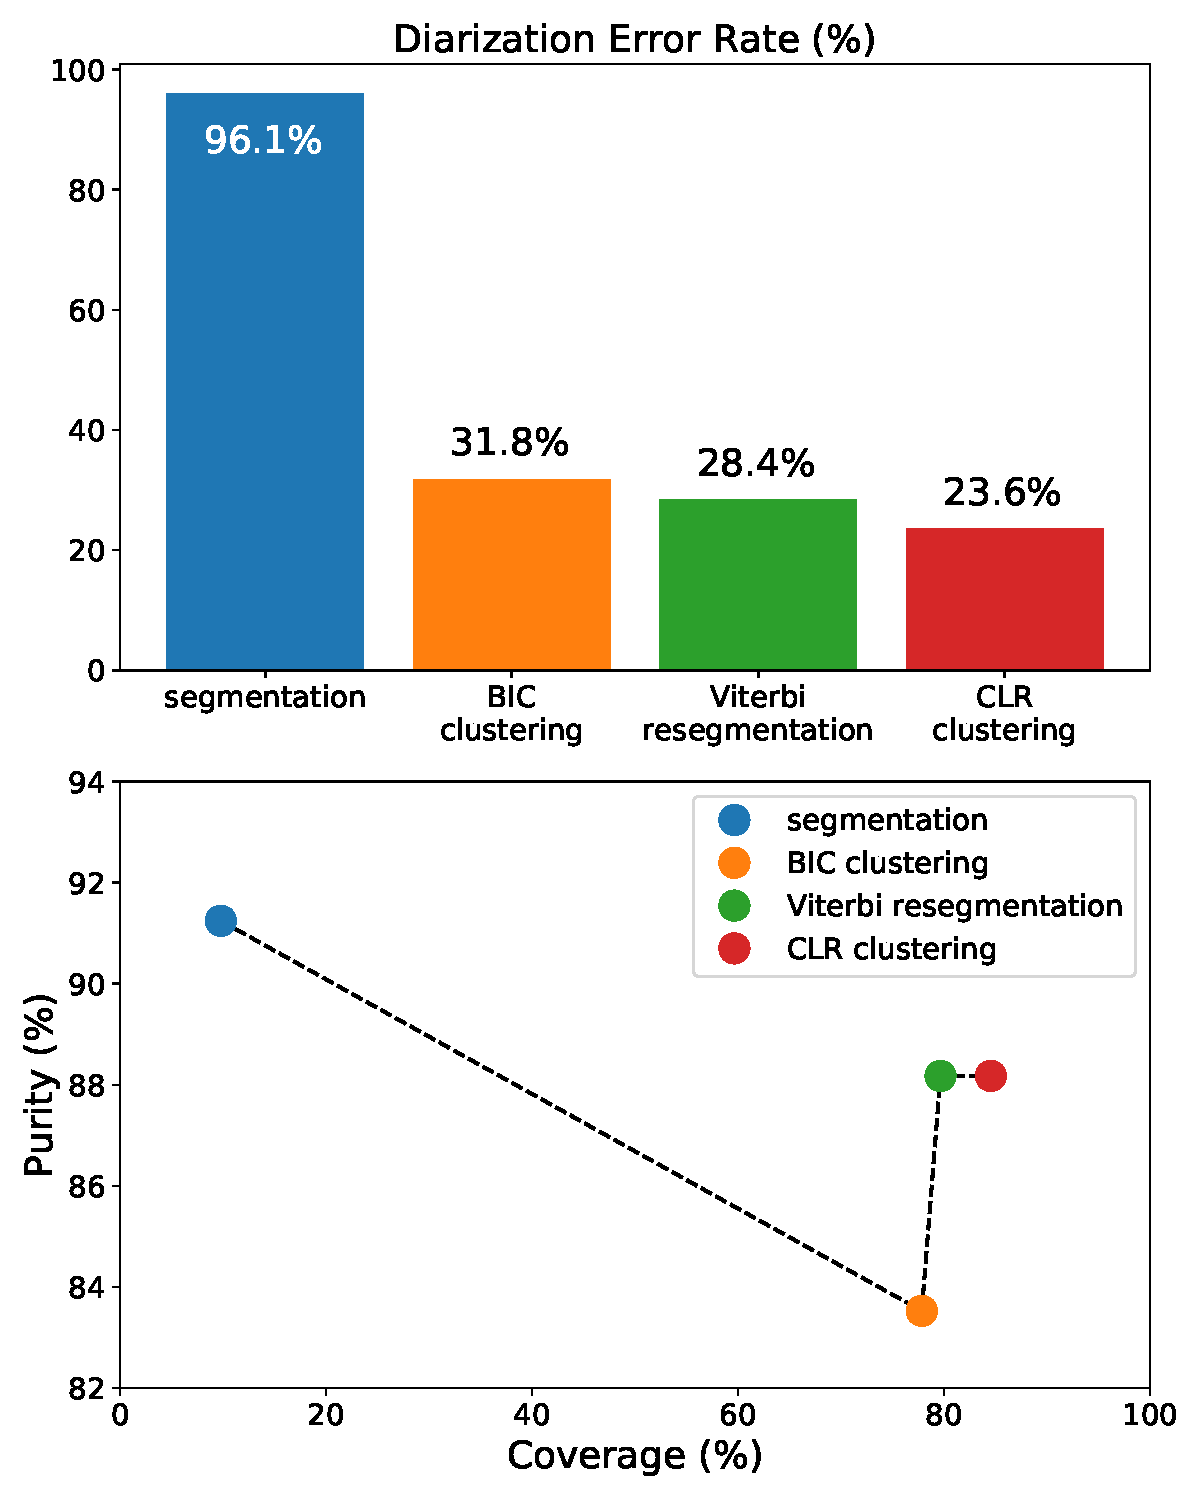
\includegraphics[width=0.8\linewidth]{figures/diagnostic.pdf}
  \caption{Diagnosing LIMSI multi-stage speaker diarization system~\cite{Barras2006}}
  \label{fig:diagnostic}
\end{figure}

Figure~\ref{fig:diagnostic} depicts the evolution of LIMSI multi-stage speaker diarization system~\cite{Barras2006} applied on the ETAPE dataset~\cite{Gravier2012}.
It is roughly made of four consecutive modules (segmentation, BIC clustering, Viterbi resegmentation, and CLR clustering).
From the upper part of the figure (DER as a function of the module), it is clear that each module improves the output of the previous one.
Yet, the lower part of the figure clarifies the role of each module.
BIC clustering tends to increase the size of the speaker clusters, at the expense of purity ($-7\%$).
Viterbi resegmentation addresses this limitation and greatly improves cluster purity ($+5\%$), with very little impact on the actual cluster coverage ($+2\%$).
Finally, CLR clustering brings an additional $+5\%$ coverage improvement.

\subsection{Identification}

In case prior speaker models are available, the speech turn clustering module in Figure~\ref{fig:pipeline} may be followed by a supervised speaker recognition module for cluster-wise supervised classification.
\texttt{pyannote.metrics} also provides a collection of evaluation metrics for this identification task. This includes precision, recall, and identification error rate (IER):

\begin{equation*}
  \text{IER} = \frac{\text{false alarm} + \text{missed detection} + \text{confusion}}{\text{total}}
\end{equation*}
which is similar to the diarization error rate (DER) introduced previously, except that the $\texttt{confusion}$ term is computed directly by comparing reference and hypothesis labels, and does not rely on a prior one-to-one matching.

\subsection{Collar and evaluation map}

Because manual annotations cannot be precise at the audio sample level, it is common in speaker diarization research to remove from evaluation a $500$ms collar around each speaker turn boundary ($250$ms before and after).
Most of the metrics available in \texttt{pyannote.metrics} support a \emph{collar} parameter, which defaults to 0.

Moreover, though audio files can always be processed entirely (from beginning to end), there are cases where reference annotations are only available for some regions of the audio files.
All metrics support the provision of an \emph{evaluation map}~\cite{NIST-RT03} that indicate which part of the audio file should be evaluated.

\section{Visual error analysis}
\label{sec:visualization}

As useful as those metrics can be, it is often necessary to have a closer look at the actual output of each module, for error analysis or visual inspection.
Existing audio annotation tools such as transcriber~\cite{transcriber} or Praat~\cite{praat} may be used for that purpose.
However, they require the researcher to generate annotation files, switch from their Python environment to a new software, and then only be able to browse and inspect the annotations.
Moreover, because they were designed for annotation purposes, they do not provide advanced functionalities to easily locate hypothesis errors.

\begin{figure}[htb]
  \centering
  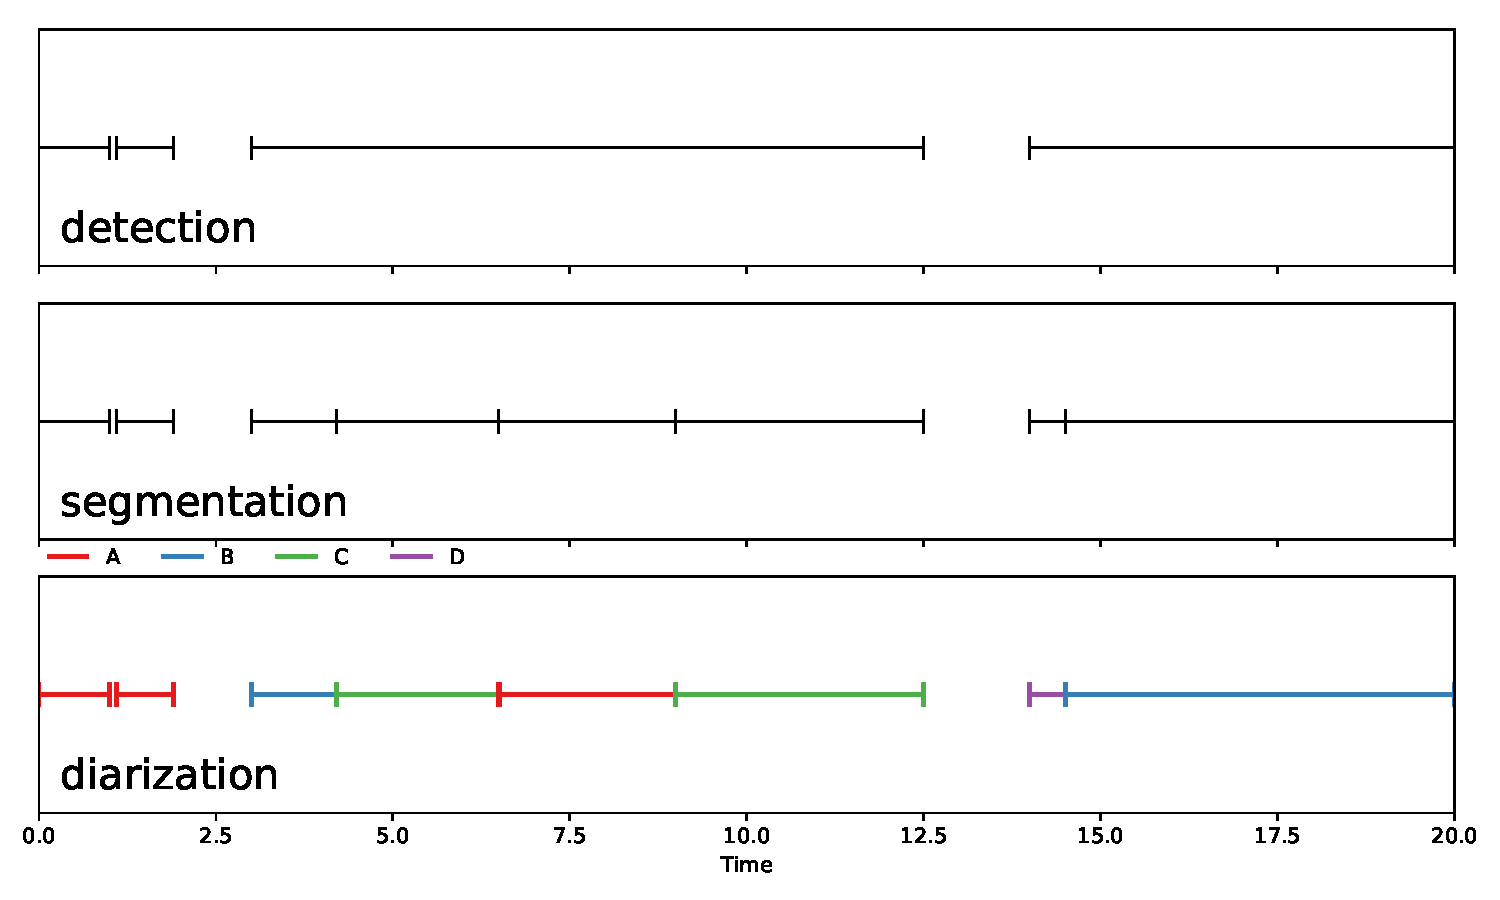
\includegraphics[width=\linewidth]{figures/visualization.pdf}
  \caption{Inspecting the output of speaker diarization modules}
  \label{fig:visualization}
\end{figure}

Because it internally relies on \texttt{pyannote.core} advanced visualization capabilities, \texttt{pyannote.metrics} addresses the first limitation. It can be used to visualize each step of any speaker diarization pipeline, without leaving the current Python or Jupyter Notebook~\cite{jupyter} environment.
Figure~\ref{fig:visualization} was obtained using this feature -- showing it can also be used to generate publication-quality figures.

\begin{figure}[htb]
  \centering
  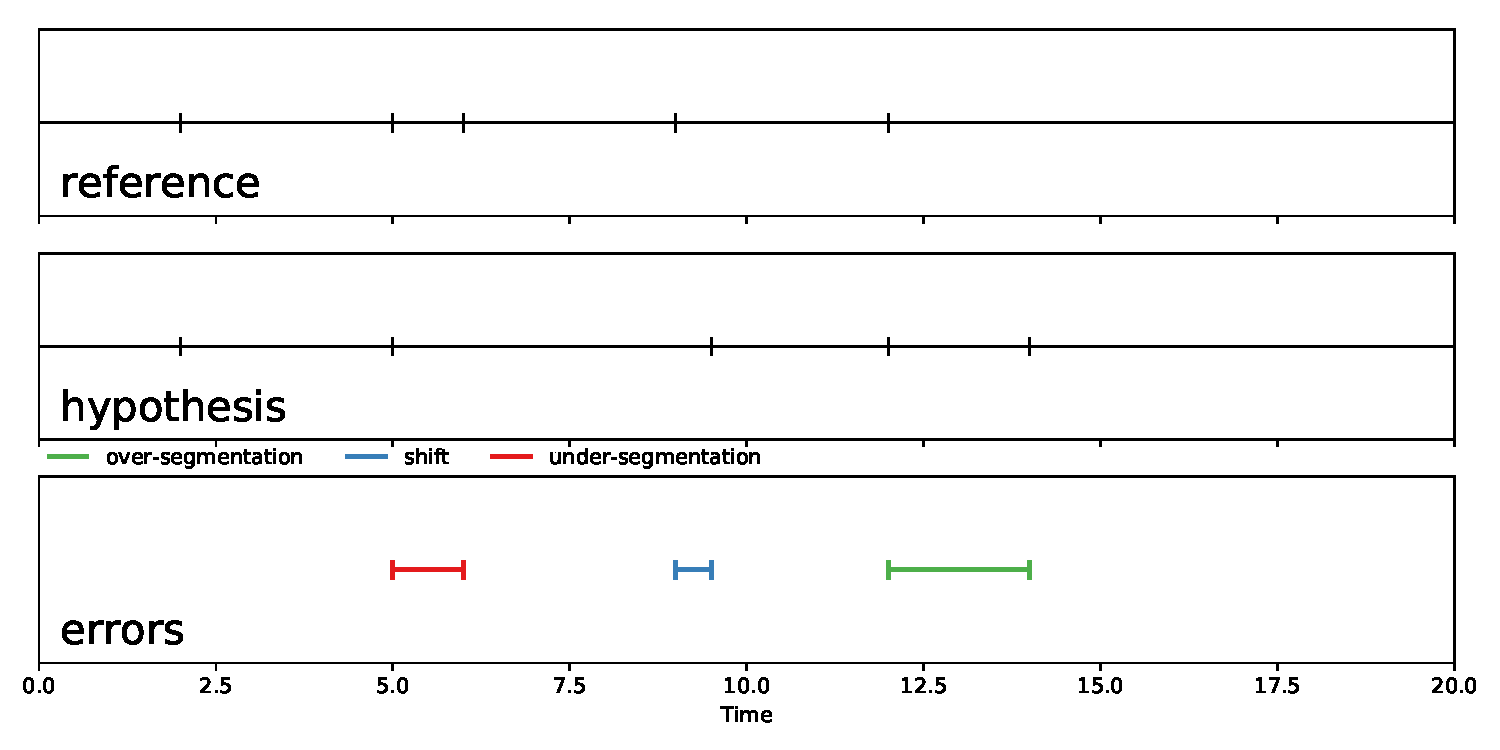
\includegraphics[width=\linewidth]{figures/segmentation_error.pdf}
  \caption{Visualizing segmentation errors}
  \label{fig:segmentation_errors}
\end{figure}

Finally, \texttt{pyannote.metrics} also provides a few tools dedicated to the analysis of segmentation or diarization errors.
Figure~\ref{fig:segmentation_errors} provides an example of segmentation error analysis.
Given a reference and hypothesized segmentations, the third line is generated automatically and allows to quickly get insight at the type and location of segmentation errors.
This example contains three errors: one boundary is not at the right location (\emph{shift} error), one boundary is missing (\emph{under-segmentation} error), and one segment is incorrecly split into two smaller ones (\emph{over-segmentation} error).

\section{Conclusion}

In this paper, we introduced \texttt{pyannote.metrics} an open-source Python library for reproducible evaluation, diagnostic, and error analysis of speaker diarization systems.
Installation instructions, example notebooks, and documentation can be found on the dedicated website \url{pyannote.github.io}.

\section{Acknowledgements}

This work was partly supported by ANR through
the ODESSA (ANR-15-CE39-0010) and MetaDaTV (ANR-14-CE24-0024) projects.


\bibliographystyle{IEEEtran}
\bibliography{mybib}

\end{document}
